\section{Aufgabenstellung}
\label{Aufgabenstellung}
%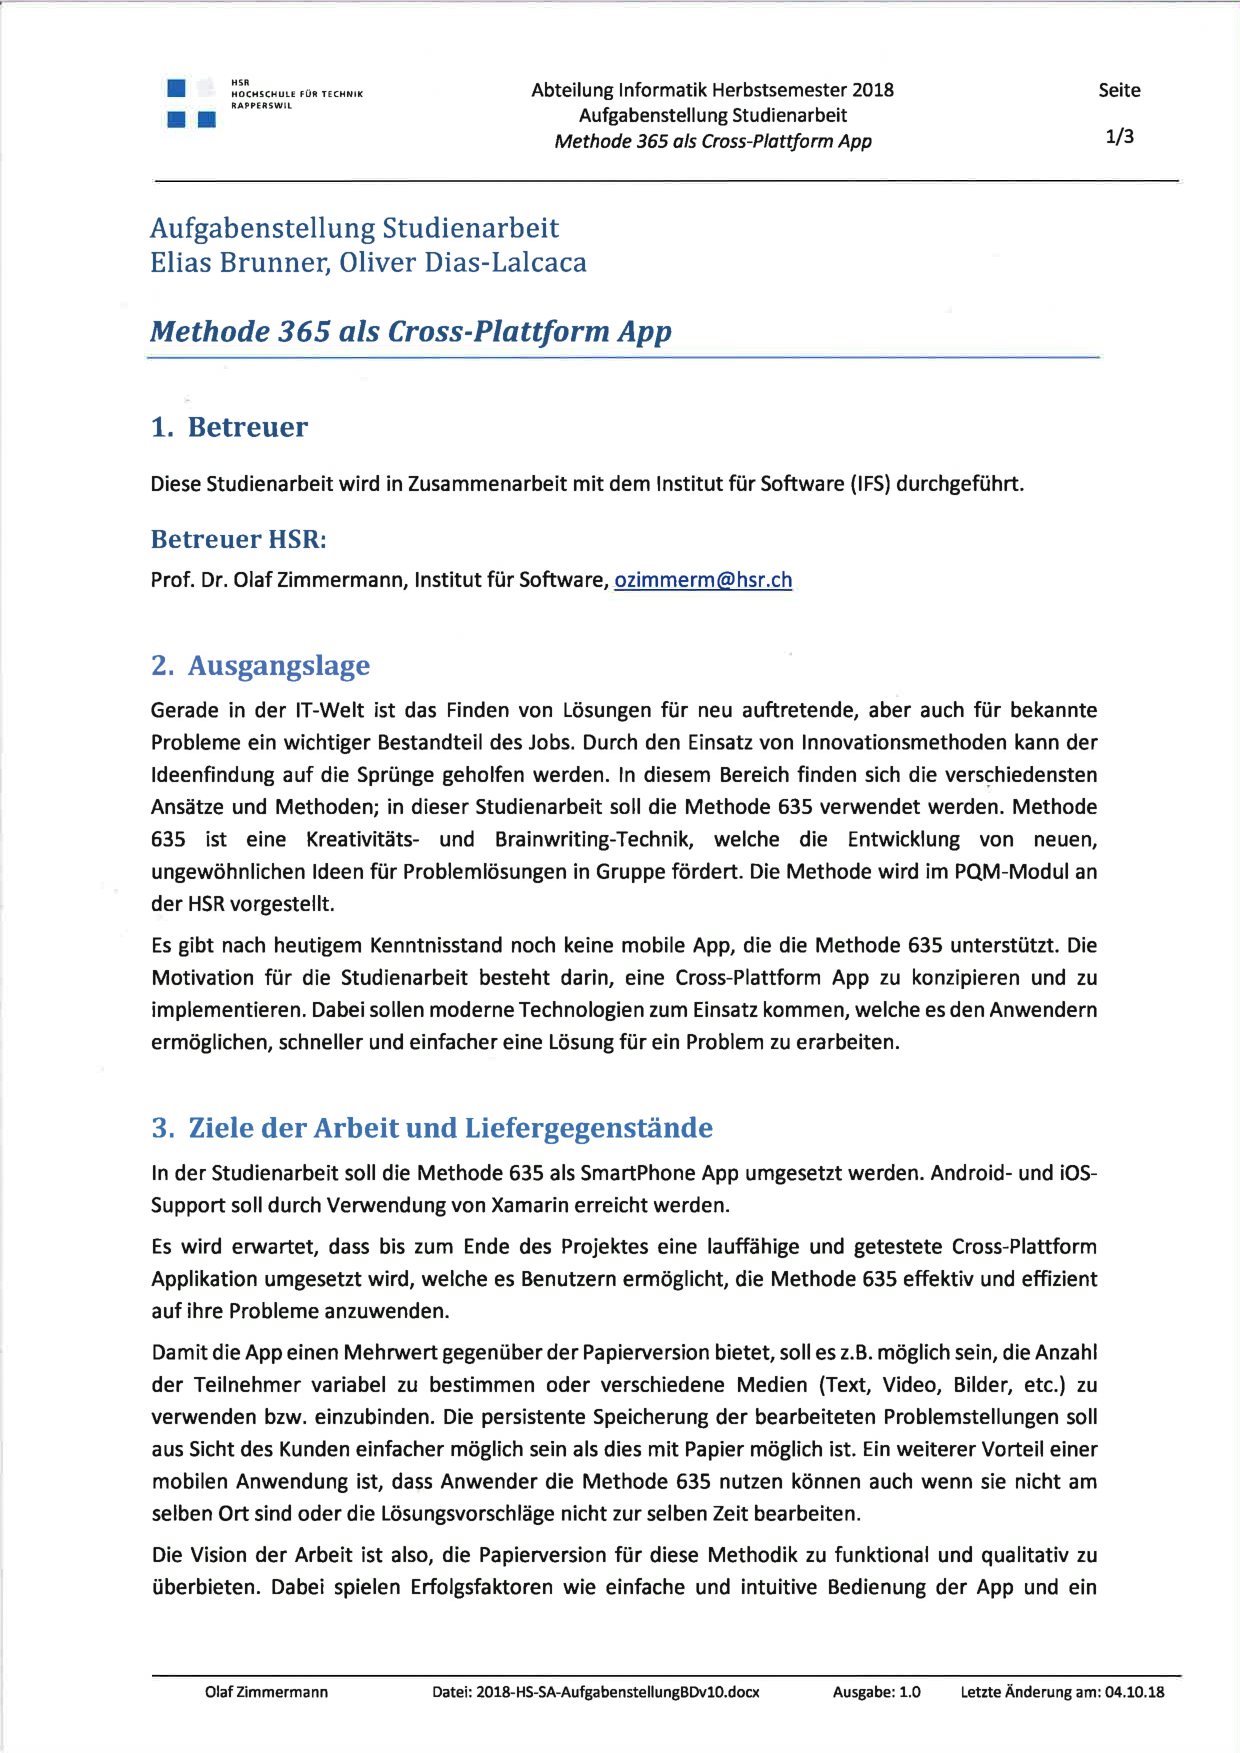
\includepdf{./res/legal/aufgabenstellung.pdf}

\subsection{Ausgangslage}
Gerade in der IT-Welt ist das Finden von Lösungen für neu auftretende, aber auch für bekannte Probleme ein wichtiger Bestandteil des Jobs. Durch den Einsatz von Innovationsmethoden kann der Ideenfindung auf die Sprünge geholfen werden. In diesem Bereich finden sich die verschiedensten Ansätze und Methoden; in dieser Studienarbeit soll die Methode 635 \cite{methode-635} verwendet werden. Methode 635 ist eine Kreativitäts- und Brainwriting-Technik, welche die Entwicklung von neuen, ungewöhnlichen Ideen für Problemlösungen in der Gruppe fördert. Die Methode wird im PQM-Modul an der HSR vorgestellt.
 
Es gibt nach heutigem Kenntnisstand noch keine mobile App, die die Methode 635 unterstützt. Die Motivation für die Studienarbeit besteht darin, eine Cross-Plattform App zu konzipieren und zu implementieren. Dabei sollen moderne Technologien zum Einsatz kommen, welche es den Anwendern ermöglichen, schneller und einfacher eine Lösung für ein Problem zu erarbeiten.

\subsection{Ziele der Arbeit und Liefergegenstände}\label{subsec:ziele}
In der Studienarbeit soll die Methode 635 als SmartPhone App umgesetzt werden. Android- und iOS- Support soll durch Verwendung von Xamarin erreicht werden.
Es wird erwartet, dass bis zum Ende des Projektes eine lauffähige und getestete Cross-Plattform Applikation umgesetzt wird, welche es Benutzern ermöglicht, die Methode 635 effektiv und effizient auf ihre Probleme anzuwenden. 

Damit die App einen Mehrwert gegenüber der Papierversion bietet, soll es z.B. möglich sein, die Anzahl der Teilnehmer variabel zu bestimmen oder verschiedene Medien (Text, Video, Bilder, etc.) zu verwenden bzw. einzubinden. Die Persistierung der bearbeiteten Problemstellungen soll aus Sicht des Kunden einfacher möglich sein als dies mit Papier möglich ist. Ein weiterer Vorteil einer mobilen Anwendung ist, dass Anwender die Methode 635 nutzen können auch wenn sie nicht am selben Ort sind oder die Lösungsvorschläge nicht zur selben Zeit bearbeiten. 

Die Vision der Arbeit ist also, die Papierversion für diese Methodik zu funktional und qualitativ zu überbieten. Dabei spielen Erfolgsfaktoren wie einfache und intuitive Bedienung der App und ein unkompliziertes Reporting sowie Robustheit und Stabilität (Bsp. keine Zeit- und Datenverluste) eine wichtige Rolle.

Weitere kritische Erfolgsfaktoren sind:
\begin{itemize}
  \item Konfigurierbarkeit (z.B. Anzahl Teilnehmer und Schritte)  und Erweiterbarkeit (im Hinblick auf Folgearbeiten, die u.U. auch andere Brainstorming Methoden unterstützen)
  \item sinnvolle Ausnutzung der Smartphone-Fähigkeiten, um einen Mehrwert im Vergleich zur traditionellen, papiergestützten Methode zu erreichen
  \item Validierung der Konzepte und ihrer Implementierung mit Hilfe von User Tests in mindestens einem Anwendungsbereich (Bsp. Architekturentscheidungen und -optionen).
\end{itemize}

